\documentclass{standalone}
\usepackage[utf8]{inputenc}
\usepackage[T1]{fontenc}
\usepackage{graphicx}
\usepackage{amsmath}
\usepackage[]{tikz, pgf}
\usetikzlibrary{arrows,shapes,calc,positioning}

\begin{document}
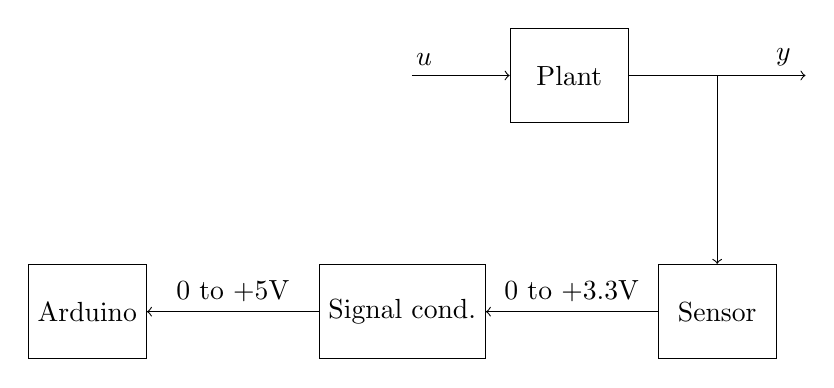
\begin{tikzpicture}[block/.style={rectangle, draw, minimum width=15mm, minimum height=12mm}, 
  node distance=40mm]
  \node[block] (sys) {Plant};
  \draw[->] (sys) ++(-20mm,0) -- node[very near start, above] {$u$} (sys);
  \draw[->] (sys) -- node[coordinate] (measure) {} node[very near end, above] {$y$} ++(3cm,0);
  \node[block, below of=measure, node distance=30mm] (sensor) {Sensor};
  \draw[->] (measure) -- (sensor);
  \node[block, left of=sensor] (cond) {Signal cond.};
  \node[block, left of=cond] (arduino) {Arduino};
  \draw[->] (sensor) -- node[above] {0 to +3.3V} (cond);
  \draw[->] (cond) -- node[above] {0 to +5V} (arduino);

\end{tikzpicture}
\end{document}
